\graphicspath{{chapters/5_experimentos/figures/}}

\chapter{Experimentación}\label{chap:experiments}

Para analizar el rendimiento de la implementación, se realizaron experimentos en distintas tarjetas gráficas, las cuales se ven en el cuadro \ref{tab:hardware-used}.
Las escenas utilizadas se muestran en las figuras \ref{fig:cornell-box-full} y \ref{fig:sponza}, las llamaremos $S1$ y $S2$ respectivamente.
Se puede observar en cada una de ellas la luz indirecta difusa, luz indirecta especular y sombras suaves.

\begin{table}[ht]
	\centering
	\begin{tabular}{|c|c|c|c|c|}
		\hline
		\textbf{Nombre} & \textbf{GPU} & \textbf{Núcleos} & \textbf{Clock (GHz)} & \textbf{VRAM (GB)} \\
		\hline
		$H1$ & Intel Mesa ADL GT2 & 96 & 1.45 & ??? \\
		\hline
		$H2$ & Nvidia GTX 1660 Ti mobile & 1536 & 1.45 & 6 \\
		\hline
		$H3$ & Nvidia Geforce RTX 4070 & 5888 & 1.92 & 12 \\
		\hline
	\end{tabular}
	\caption{Hardware utilizado.}
	\label{tab:hardware-used}
\end{table}

\begin{figure}[ht]
	\centering
    \begin{subfigure}{1.0\textwidth}
        \centering
		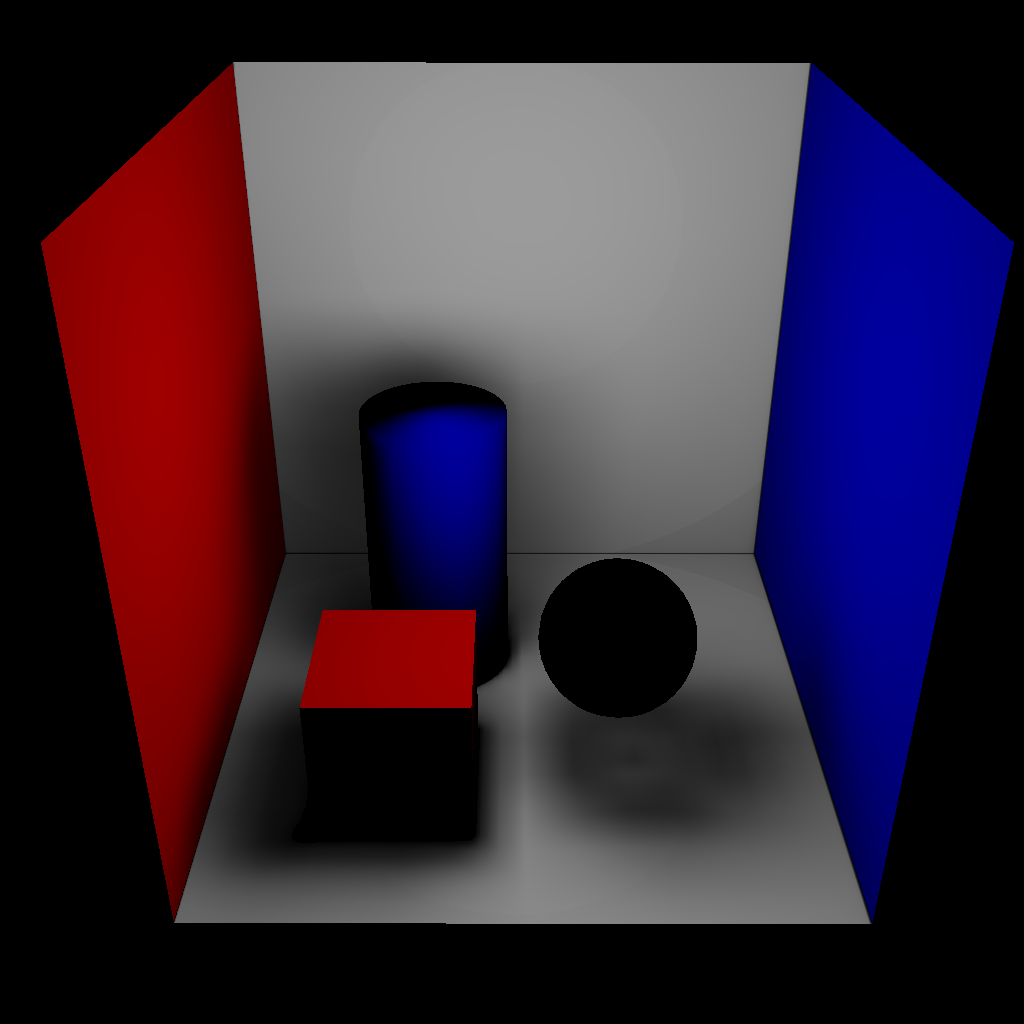
\includegraphics[width=0.7\textwidth]{cornell-box-direct.png}
        \caption{Solo luz directa.}
    \end{subfigure}
    \begin{subfigure}{1.0\textwidth}
        \centering
		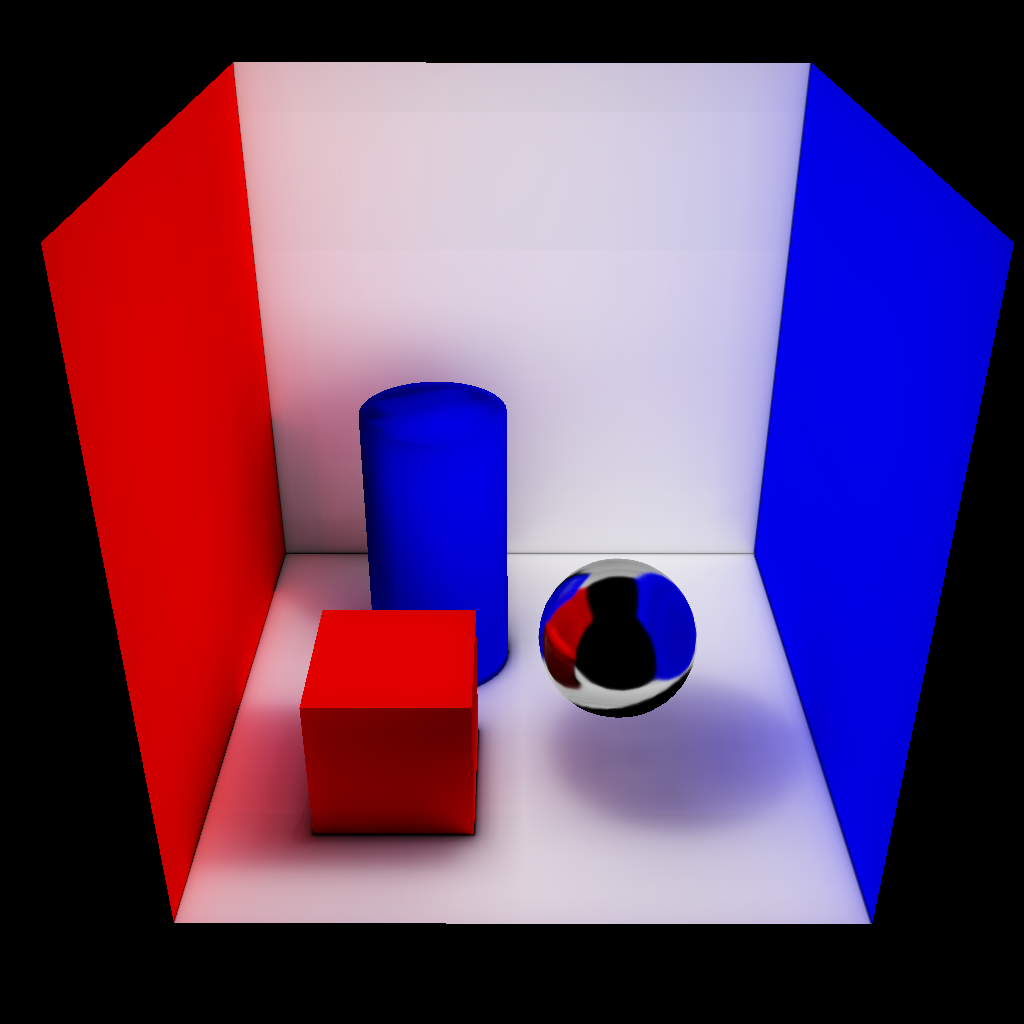
\includegraphics[width=0.7\textwidth]{cornell-box-full.png}
        \caption{Luz directa e indirecta.}
    \end{subfigure}
	\caption{Escena de prueba con geometría simple.}
	\label{fig:cornell-box-full}
\end{figure}

\begin{figure}[ht]
	\begin{subfigure}{.49\textwidth}
		\centering
		\includegraphics[width=\textwidth]{sponza-direct.png}
		\caption{Solo luz directa.}
	\end{subfigure}
	\begin{subfigure}{.49\textwidth}
		\centering
		\includegraphics[width=\textwidth]{sponza-all.png}
		\caption{Luz directa e indirecta.}
	\end{subfigure}
	\caption{Sponza.}
	\label{fig:sponza}
\end{figure}

Los experimentos varían la cantidad de vóxeles por dimensión, y registran los cuadros por segundo alcanzados (FPS, por sus siglas en inglés) y el tiempo de construcción del \textit{octree} en segundos.
Para conseguir los FPS se ejecutó el programa durante un minuto, tomando una muestra cada segundo, luego se promediaron.
Para el tiempo de construcción del \textit{octree}, se construyó 50 veces y se calculó el tiempo promedió.
Cada ejecución se realizó independientemente, para evitar posibles mejoras debido al uso del cache.

En las tablas \ref{tab:cisco-laptop}, \ref{tab:pizzo-laptop} y \ref{tab:pizzo-desktop} se muestran los resultados de estos experimentos en tarjetas Intel Mesa ADL GT2 integrada de laptop, Nvidia GTX 1660 Ti de laptop y Nvidia RTX 4070 respectivamente.
En cada tabla se muestran los resultados para cada una de las escenas $S1$ y $S2$.

\begin{table}[ht]
\centering
\begin{tabular}{|c|c|c|c|}
	\hline
	\textbf{Vóxeles} & \textbf{Escena} & \textbf{FPS} & \textbf{Construcción del \textit{octree} (s)} \\
	\hline
	$256$ & $S1$ & $14.47$ & $4.62$ \\
	 & $S2$ & $17.05$ & $3.82$ \\
	\hline
	$512$ & $S1$ & $11.30$ & $5.04$ \\
	 & $S2$ & $14.08$ & $3.66$ \\
	\hline
	$1024$ & $S1$ & $9.22$ & $4.40$ \\
	 & $S2$ & $12.57$ & $3.78$ \\
	\hline
\end{tabular}
\caption{Experimentos usando $H1$.}
\label{tab:cisco-laptop}
\end{table}

\begin{table}[hb]
\centering
\begin{tabular}{|c|c|c|c|}
	\hline
	\textbf{Vóxeles} & \textbf{Escena} & \textbf{FPS} & \textbf{Construcción del \textit{octree} (s)} \\
	\hline
	$256$ & $S1$ & $13.70$ & $2.46$ \\
	 & $S2$ & $13.79$ & $2.48$ \\
	\hline
	$512$ & $S1$ & $11.87$ & $2.63$ \\
	 & $S2$ & $11.92$ & $2.57$ \\
	\hline
	$1024$ & $S1$ & $10.58$ & $2.96$ \\
	 & $S2$ & $10.65$ & $2.92$ \\
	\hline
\end{tabular}
\caption{Experimentos usando $H2$.}
\label{tab:pizzo-laptop}
\end{table}

\begin{table}[hb]
\centering
\begin{tabular}{|c|c|c|c|}
	\hline
	\textbf{Vóxeles} & \textbf{Escena} & \textbf{FPS} & \textbf{Construcción del \textit{octree} (s)} \\
	\hline
	$256$ & $S1$ & $141.57$ & $1.88$ \\
	 & $S2$ & 141.59 & 1.90 \\
	\hline
	$512$ & $S1$ & $141.47$ & $1.90$ \\
	 & $S2$ & $141.51$ & $1.91$ \\
	\hline
	$1024$ & $S1$ & $140.88$ & $1.89$ \\
	 & $S2$ & $141.21$ & $1.99$ \\
	\hline
\end{tabular}
\caption{Experimentos usando $H3$.}
\label{tab:pizzo-desktop}
\end{table}

\section{Análisis de resultados}

Una observación es la falta de rendimiento, dado que en las tarjetas gráficas de laptops en las que se ejecutó, se consiguieron muy pocos cuadros por segundo y en todas las tarjetas los tiempos de construcción del octree fueron muy altos.
Los valores de estas métricas son mucho mejores en el artículo original del algoritmo, en el que se mostraron entre 20 y 30 cuadros por segundo y 280 milisegundos de construcción del \textit{octree}, en lugar de segundos.

Una observación es que la tarjeta Nvidia RTX 4070 trae excelentes resultados en terminos de cuadros por segundo, pero sorprendentemente es más lenta que la Intel Mesa ADL GT2 en construír el \textit{octree}.
Esto puede deberse a que la primer tarjeta posee mucho más paralelización, por lo que puede realizar todos los trazados de conos sin problemas, pero este no es el cuello de botella para la construcción del \textit{octree}, sino la comunicación entre CPU y GPU.

Fingxels logró correr escenas a aproximadamente 15 FPS en tarjetas gráficas de laptops, mientras que el artículo original logró aproximadamente 30 FPS.
En una tarjeta de última generación se lograron aproximadamente 140 FPS.
Sin embargo, el tiempo de construcción de la estructura de datos fue mucho más lento que en el trabajo original para todas las tarjetas probadas.
